\documentclass[tikz,border=8pt]{standalone}
% Shared look for every TikZ diagram. Load with \input{../../tools/tikz-style.tex}
\usepackage[T1]{fontenc}
\usepackage{lmodern}
\renewcommand{\sfdefault}{lmr}  % diagrams use the same serif as the text
\usetikzlibrary{arrows.meta, positioning, shapes.geometric, calc, fit, backgrounds}
\definecolor{cblue}{HTML}{4C78A8}
\definecolor{corange}{HTML}{F58518}
\definecolor{cgreen}{HTML}{54A24B}
\definecolor{cred}{HTML}{E45756}
\definecolor{cpurple}{HTML}{B279A2}
\definecolor{cgrey}{HTML}{6B6B6B}
\tikzset{
  every picture/.style={font=\sffamily, line width=1.2pt},
  box/.style={draw=#1, fill=#1!12, rounded corners=4pt, align=center, inner sep=7pt, minimum height=1.1cm},
  box/.default=cgrey,
  arrow/.style={-{Stealth[length=3mm]}, draw=cgrey, line width=1.4pt},
  title/.style={font=\sffamily\bfseries\Large},
  note/.style={font=\sffamily\small, text=cgrey, align=center},
}
\AtBeginDocument{\hyphenpenalty=10000 \exhyphenpenalty=10000}

\begin{document}
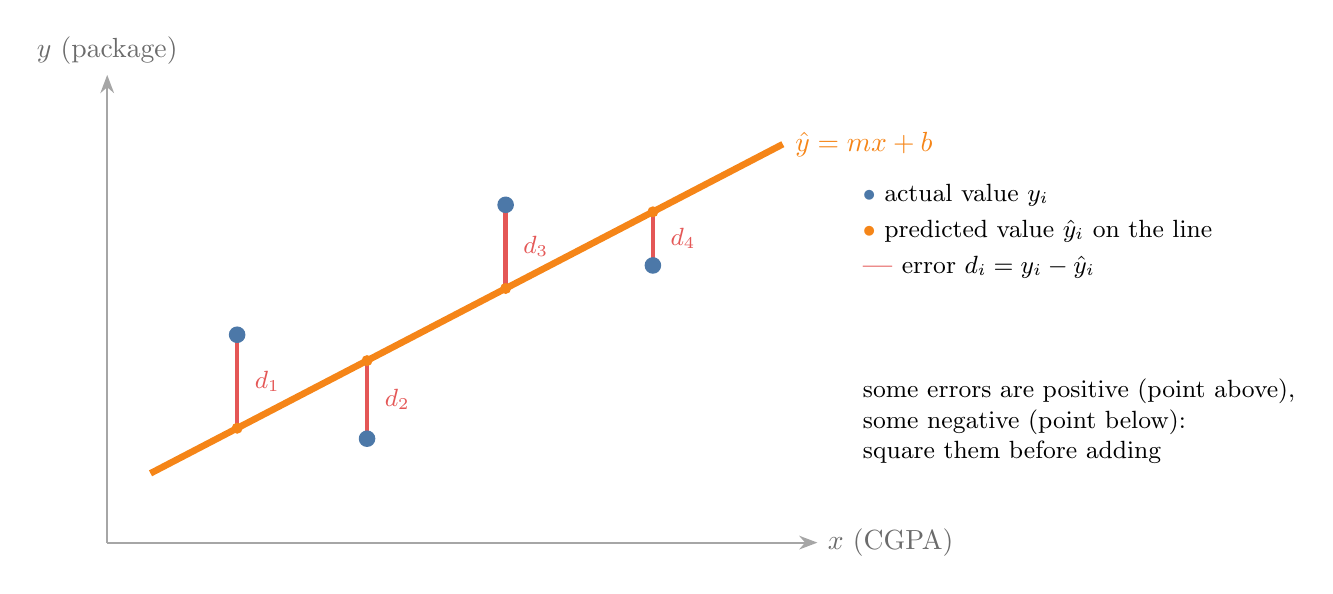
\begin{tikzpicture}[x=1.1cm,y=1.1cm]
  \draw[cgrey!60, line width=0.8pt, -{Stealth}] (0,0) -- (8.2,0) node[right, text=cgrey] {$x$ (CGPA)};
  \draw[cgrey!60, line width=0.8pt, -{Stealth}] (0,0) -- (0,5.4) node[above, text=cgrey] {$y$ (package)};
  \draw[corange, line width=2.4pt] (0.5,0.8) -- (7.8,4.6) node[right, font=\bfseries] {$\hat{y} = mx + b$};
  \foreach \x/\y/\n in {1.5/2.4/1, 3/1.2/2, 4.6/3.9/3, 6.3/3.2/4} {
    \pgfmathsetmacro{\yh}{0.8+(\x-0.5)*3.8/7.3}
    \draw[cred, line width=1.6pt] (\x,\y) -- (\x,\yh);
    \fill[cblue] (\x,\y) circle (3pt);
    \fill[corange] (\x,\yh) circle (2pt);
    \node[font=\small, text=cred, anchor=west] at (\x+0.08,{(\y+\yh)/2}) {$d_{\n}$};
  }
  \node[anchor=west, align=left, font=\small] at (8.6,3.6) {\textcolor{cblue}{$\bullet$} actual value $y_i$\\[2pt]\textcolor{corange}{$\bullet$} predicted value $\hat{y}_i$ on the line\\[2pt]\textcolor{cred}{\textbf{|}} error $d_i = y_i - \hat{y}_i$};
  \node[anchor=west, align=left, font=\small] at (8.6,1.4) {some errors are positive (point above),\\some negative (point below):\\square them before adding};
\end{tikzpicture}
\end{document}
